\documentclass[11pt,aspectratio=169]{beamer}

\usepackage{fontspec}
\usepackage[spanish,es-noindentfirst]{babel}
\usepackage{graphicx}
\usepackage{booktabs}
\usepackage{xcolor}

\definecolor{azulucuenca}{RGB}{0,42,84}
\definecolor{rojoucuenca}{RGB}{180,30,30}
\definecolor{grisucuenca}{RGB}{90,90,90}

\usetheme{default}
\usecolortheme[named=azulucuenca]{structure}
\setbeamercolor{title}{fg=white,bg=azulucuenca}
\setbeamercolor{frametitle}{fg=white,bg=azulucuenca}
\setbeamercolor{block title}{fg=white,bg=rojoucuenca}
\setbeamercolor{block body}{fg=black,bg=azulucuenca!6}
\setbeamertemplate{navigation symbols}{}
\setbeamertemplate{footline}[frame number]
\setbeamerfont{frametitle}{series=\bfseries}

\graphicspath{{../analisis/figuras/}}
\sloppy

\title{Análisis de Redes Complejas}
\subtitle{Caso de estudio: la red de datos de la Universidad de Cuenca}
\author{Efrain Adolfo Alvarado Plasencia}
\institute{Maestría en Ciencias de la Ingeniería Eléctrica --- Módulo 1217, Redes Complejas\\
\texttt{efrain.alvarado@ucuenca.edu.ec}}
\date{Agosto de 2026}

\begin{document}

% ---------------------------------------------------------------
\begin{frame}
\titlepage
\end{frame}

% ---------------------------------------------------------------
\begin{frame}{La pregunta que guía el proyecto}
\begin{block}{}
\centering\Large
¿Cuáles son los puntos críticos de la red de datos de la\\
Universidad de Cuenca, qué tan grave sería su falla, y qué\\
intervenciones concretas mejorarían más su robustez y desempeño?
\end{block}
\vfill
\begin{itemize}
  \item Red real de infraestructura: 177 equipos, 209 enlaces, 6 campus
  \item Reconstruida a partir de 34 diagramas del informe técnico institucional
  \item Cinco fases del módulo, encadenadas sobre el mismo grafo
\end{itemize}
\end{frame}

% ---------------------------------------------------------------
\begin{frame}{El caso de estudio}
\begin{columns}[T]
\begin{column}{0.5\textwidth}
\textbf{Jerarquía de tres capas:}
\begin{itemize}
  \item \emph{Core}: 5 nodos
  \item Agregación: 27 nodos
  \item Acceso: 132 nodos
  \item WAN / interconexión: 13 nodos
\end{itemize}
\vspace{4mm}
\textbf{Seis campus} conectados por una nube MPLS:\\
Central, Balzay, Paraíso, Yanuncay, Hospitalidad + 2 sedes menores
\end{column}
\begin{column}{0.5\textwidth}
\centering
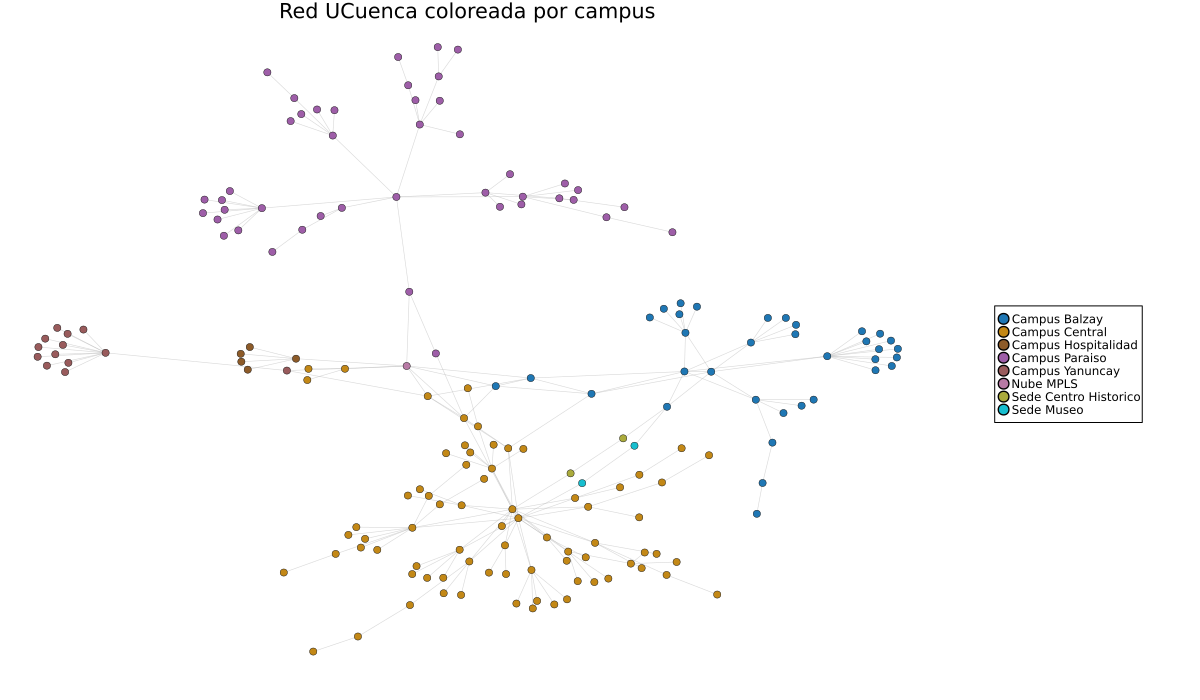
\includegraphics[width=\textwidth]{p2_red_por_campus.png}
\end{column}
\end{columns}
\end{frame}

% ---------------------------------------------------------------
\begin{frame}{Metodología}
\begin{enumerate}
  \item \textbf{Caracterización} --- medidas estructurales, modelos nulos
  \item \textbf{Recorrido y partición} --- BFS/DFS, comunidades (Louvain)
  \item \textbf{Optimización} --- caminos mínimos, flujo máximo, localización
  \item \textbf{Percolación y robustez} --- fallos, cascadas, epidemias
  \item \textbf{Propuesta de rediseño} --- intervenciones acotadas y cuantificadas
\end{enumerate}
\vfill
\begin{block}{Reproducibilidad}
Código en Julia (\texttt{analisis/scripts/}), reutiliza el código base y el
código de referencia del módulo (Ford-Fulkerson, Edmonds-Karp, \emph{k}-means).
Los 5 scripts corren de punta a punta sin intervención manual.
\end{block}
\end{frame}

% ---------------------------------------------------------------
\begin{frame}{Fase 1 --- Caracterización estructural}
\begin{columns}[T]
\begin{column}{0.55\textwidth}
\begin{itemize}
  \item Densidad 0{,}013 --- red muy dispersa
  \item Clustering 0{,}095, asortatividad $-0{,}147$: jerarquía \emph{core}-agregación-acceso, no red social
  \item \textbf{47 puntos de articulación}
  \item \textbf{141 puentes (67{,}5\,\%)} de los enlaces
\end{itemize}
\vspace{3mm}
\begin{block}{Contraste con el informe técnico}
El informe afirma redundancia \emph{core}-agregación en Balzay \textbf{y Paraíso}.
Los datos confirman Balzay pero \textbf{refutan Paraíso}: agregación de
puertos hacia un único \emph{core}, no redundancia real.
\end{block}
\end{column}
\begin{column}{0.45\textwidth}
\centering
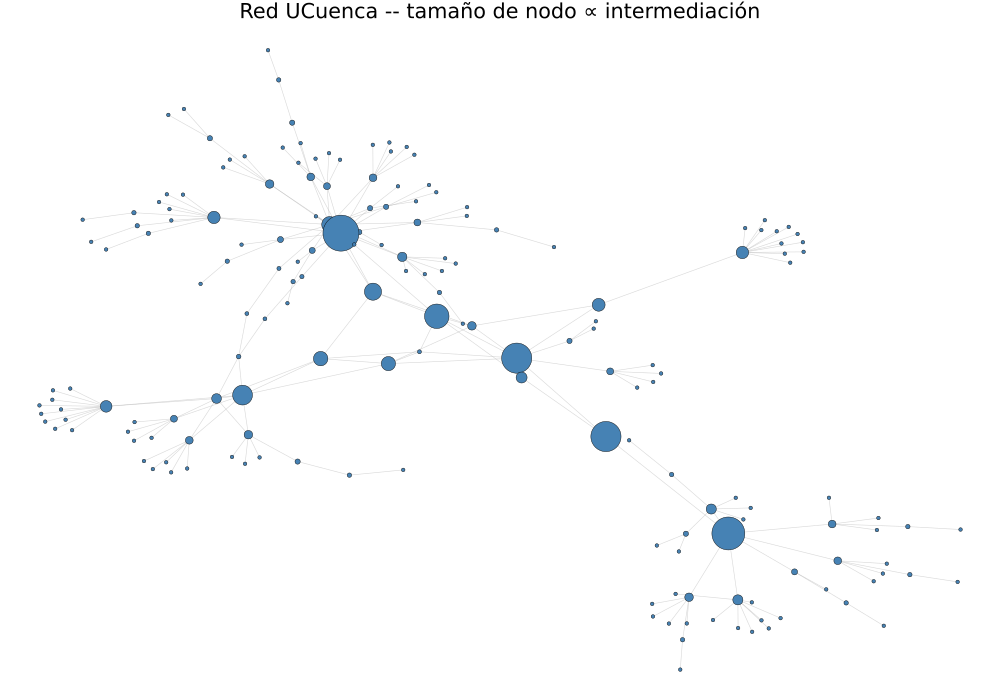
\includegraphics[width=\textwidth]{p2_red_por_intermediacion.png}
\end{column}
\end{columns}
\end{frame}

% ---------------------------------------------------------------
\begin{frame}{Fase 2 --- Comunidades}
\begin{columns}[T]
\begin{column}{0.55\textwidth}
\begin{itemize}
  \item Louvain (implementado desde cero): \textbf{22 comunidades}, $Q=0{,}75$
  \item Estable en 5 semillas (NMI $\geq0{,}93$ entre corridas)
  \item Vs.\ partición por campus: NMI$=0{,}58$, ARI$=0{,}19$
  \item Louvain no mezcla campus, pero sí subdivide cada uno --- casi bloque-diagonal
\end{itemize}
\end{column}
\begin{column}{0.45\textwidth}
\begin{block}{Un hallazgo concreto}
11 equipos (casi todos WAN: \texttt{INTERNET-MPLS},\\ \texttt{PE1/PE2-CENTRAL}, \texttt{FORTIGATE-CENTRAL}\ldots) quedan agrupados con Balzay --- Louvain detecta un \textbf{``núcleo WAN''} como bloque funcional propio.
\end{block}
\end{column}
\end{columns}
\end{frame}

% ---------------------------------------------------------------
\begin{frame}{Fase 3 --- El hallazgo central: Campus Paraíso}
\begin{columns}[T]
\begin{column}{0.55\textwidth}
\textbf{Flujo máximo hacia Internet/MPLS, por campus:}
\begin{table}
\small
\begin{tabular}{lrr}
\toprule
Campus & Acceso & Flujo máx.\ \\
\midrule
Central & 56 & 44\,000 Mbps \\
Balzay & 24 & 23\,000 Mbps \\
Yanuncay & 11 & 10\,000 Mbps \\
Hospitalidad & 4 & 4\,000 Mbps \\
\textbf{Paraíso} & \textbf{35} & \textbf{1\,000 Mbps} \\
\bottomrule
\end{tabular}
\end{table}
\end{column}
\begin{column}{0.45\textwidth}
\begin{block}{35 equipos, un solo salto de 1 Gbps}
El corte mínimo de Paraíso es \textbf{una única arista}
(\texttt{CPAR-C10}--\texttt{ROUTER-HUAYNA-CAPAC}) --- y también es un puente
de la Fase 1. El cuello de botella físico y el punto de fragilidad
topológica \textbf{coinciden exactamente}.
\end{block}
\end{column}
\end{columns}
\end{frame}

% ---------------------------------------------------------------
\begin{frame}{Fase 3 --- Caminos mínimos y localización (resumen)}
\begin{columns}[T]
\begin{column}{0.5\textwidth}
\textbf{P5 --- Caminos más cortos}
\begin{itemize}
  \item Dijkstra (montículo propio) y Floyd-Warshall desde cero, coinciden en 20 pares al azar
  \item 3 modelos de peso: saltos, latencia estimada, carga relativa
  \item Ningún modelo produce pesos negativos
\end{itemize}
\end{column}
\begin{column}{0.5\textwidth}
\textbf{P7 --- Localización de instalaciones}
\begin{itemize}
  \item $p$-mediana / $p$-centro: heurística voraz vs.\ ILP (JuMP+HiGHS)
  \item La heurística iguala al óptimo en $p=5$
  \item Los nodos óptimos \textbf{no} son los de mayor grado/intermediación
\end{itemize}
\end{column}
\end{columns}
\end{frame}

% ---------------------------------------------------------------
\begin{frame}{Fase 4 --- La paradoja de la robustez}
\begin{columns}[T]
\begin{column}{0.5\textwidth}
\centering
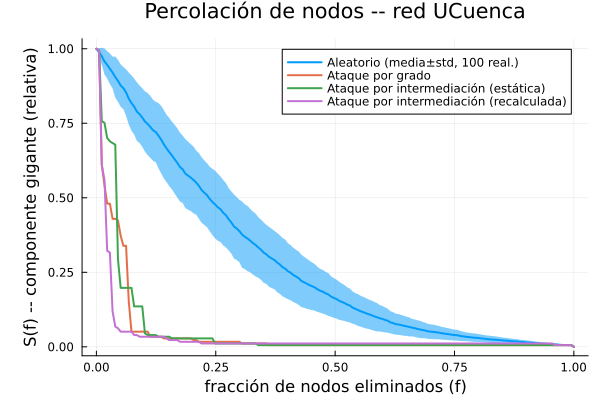
\includegraphics[width=\textwidth]{p8_percolacion_nodos.png}
\end{column}
\begin{column}{0.5\textwidth}
\textbf{Umbral de percolación $f_c$:}
\begin{itemize}
  \item Fallo aleatorio: $f_c\approx0{,}237$
  \item Ataque por grado: $f_c\approx0{,}023$
  \item Ataque por intermediación: $f_c\approx0{,}045$
\end{itemize}
\vspace{3mm}
\begin{block}{Consecuencia operativa}
Mantenimiento $\to$ tratar fallos como aleatorios (tolerancia alta).\\
Seguridad $\to$ los nodos de mayor grado necesitan protección
\textbf{desproporcionada} a su número.
\end{block}
\end{column}
\end{columns}
\end{frame}

% ---------------------------------------------------------------
\begin{frame}{Fase 4 --- Cascadas, epidemias e inmunización}
\begin{itemize}
  \item \textbf{Cascadas (Motter-Lai)}: ningún nodo, ni con margen $\tau=0$,
    desencadena una cascada $>20$\,\% de la red --- fragilidad de
    \emph{conectividad}, no de \emph{sobrecarga en cadena}
  \item \textbf{SIR}: $\lambda_c=\langle k\rangle/\langle k^2\rangle=0{,}186$;
    tamaño del brote crece con $\lambda/\lambda_c$, coherente con la teoría
  \item \textbf{Inmunización} (mismo presupuesto, 11 equipos):
\end{itemize}
\begin{table}
\centering\small
\begin{tabular}{lrr}
\toprule
Estrategia & Tamaño del brote & Reducción \\
\midrule
Aleatoria & 36{,}1\,\% & 11{,}0\,\% \\
\textbf{Por centralidad} & \textbf{9{,}2\,\%} & \textbf{77{,}2\,\%} \\
\bottomrule
\end{tabular}
\end{table}
\end{frame}

% ---------------------------------------------------------------
\begin{frame}{Fase 4 --- Ranking de puntos críticos (P10)}
\small
\begin{table}
\begin{tabular}{lllc}
\toprule
Id & Campus & Capa & Índice \\
\midrule
\texttt{INTERNET-MPLS} & Nube MPLS & wan & \textbf{0{,}682} \\
\texttt{BAL-AUL2-D1} & Balzay & agregación & 0{,}585 \\
\texttt{DATCC-2A-C3} & Central & core & 0{,}530 \\
\texttt{CPAR-C10} & Paraíso & core & 0{,}524 \\
\texttt{ROUTER-HUAYNA-CAPAC} & Paraíso & wan & 0{,}503 \\
\bottomrule
\end{tabular}
\end{table}
\vspace{2mm}
Índice = promedio de intermediación + articulación + participación en
cortes mínimos (P6) + daño en cascada (P9), todos normalizados.
\end{frame}

% ---------------------------------------------------------------
\begin{frame}{Fase 5 --- Cinco intervenciones propuestas}
\scriptsize
\begin{table}
\begin{tabular}{p{2.6cm}p{5.3cm}c}
\toprule
Enlace & Justificación & Cap. \\
\midrule
\textbf{Duplicar} CPAR-C10 -- ROUTER-HUAYNA-CAPAC & Cuello de botella de flujo más severo (Paraíso) & 10\,000 \\
\textbf{Nuevo} HOS-0A-D05 -- FORTIGATE-CENTRAL & Hospitalidad: único enlace inferido a MPLS & 1\,000 \\
\textbf{Nuevo} CCJ-CJURIDICO-D4 -- DATCC-2A-C2 & Consultorio Jurídico: mismo patrón & 1\,000 \\
\textbf{Nuevo} ROUTER-YANUNCAY -- DATCC-2A-C3 & Yanuncay: único enlace troncal & 10\,000 \\
\textbf{Nuevo} AUL2-0A-A121 -- BAL-CENTEC-D2 & Mitigación puntual en Balzay & 1\,000 \\
\bottomrule
\end{tabular}
\end{table}
\normalsize
Derivadas directamente del diagnóstico de las fases 1, 3 y 4 --- no de un
criterio genérico.
\end{frame}

% ---------------------------------------------------------------
\begin{frame}{Fase 5 --- Resultado, y comparación con alternativas}
\begin{columns}[T]
\begin{column}{0.55\textwidth}
\centering
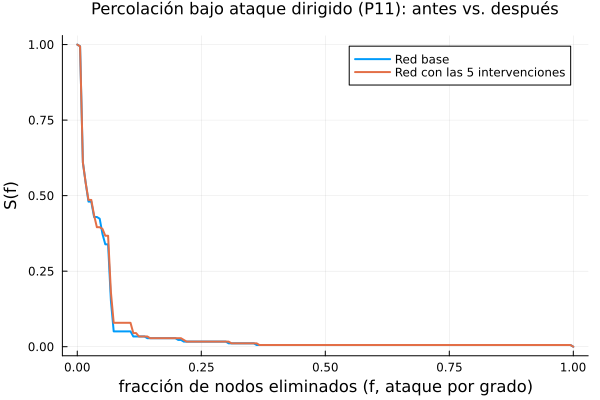
\includegraphics[width=\textwidth]{p11_percolacion_antes_despues.png}
\end{column}
\begin{column}{0.45\textwidth}
\begin{itemize}
  \item Flujo máx.\ Paraíso: \textbf{1\,000 $\to$ 10\,000 Mbps} ($+900$\,\%)
  \item Puentes: $-3$ ($-2{,}1$\,\%) --- Articulación: $-1$
  \item Eficiencia global: $+3{,}5$\,\%
\end{itemize}
\vspace{2mm}
\begin{block}{vs.\ alternativas ingenuas}
``Unir los 2 nodos de mayor grado'' y ``5 enlaces al azar'' \textbf{no}
tocan Paraíso ni Hospitalidad de forma efectiva: el mejor resultado
alternativo llega a solo 2\,000 Mbps.
\end{block}
\end{column}
\end{columns}
\end{frame}

% ---------------------------------------------------------------
\begin{frame}{Conclusiones}
\begin{enumerate}
  \item Jerarquía dispersa, poco clustering, explicada por heterogeneidad de grado
  \item Robusta ante fallos aleatorios, \textbf{frágil} ante ataques dirigidos
  \item El informe técnico \textbf{sobreestima} la redundancia de Campus Paraíso
  \item Un índice compuesto confirma consistentemente los mismos puntos críticos
  \item 5 intervenciones acotadas multiplican por 10 el flujo del campus más
    vulnerable, superando a alternativas ingenuas
\end{enumerate}
\vfill
\begin{block}{Recomendación}
\centering\Large Si hay presupuesto para 5 enlaces: \textbf{empezar por Campus Paraíso.}
\end{block}
\end{frame}

% ---------------------------------------------------------------
\begin{frame}
\centering
\vspace{1cm}
{\Huge\bfseries\color{azulucuenca} ¡Gracias!}\\[8mm]
{\Large Preguntas}\\[15mm]
{\large Efrain Adolfo Alvarado Plasencia}\\
\texttt{efrain.alvarado@ucuenca.edu.ec}\\[3mm]
\url{https://github.com/chino111160/redes-complejas-ucuenca}
\end{frame}

\end{document}
